\documentclass{standalone}
\usepackage{amsmath,amssymb}
\usepackage{newtxtext,newtxmath}
\usepackage{xcolor}
\usepackage{tikz}
\usetikzlibrary{arrows.meta,positioning,calc,decorations.pathreplacing}

\definecolor{ink}{HTML}{1B1F23}
\definecolor{slate}{HTML}{555E68}
\definecolor{muted}{HTML}{8E96A0}
\definecolor{light}{HTML}{C6CCD2}
\definecolor{faint}{HTML}{E6E9ED}
\definecolor{quantum}{HTML}{2C5E8A}
\definecolor{quantumlight}{HTML}{6C9AC3}
\definecolor{quantumpale}{HTML}{DCE7F2}
\definecolor{ochre}{HTML}{B86B19}
\definecolor{ochrelight}{HTML}{E2B98B}
\definecolor{ochrepale}{HTML}{F6E9D8}

\newcommand{\pfmain}[1]{{\fontsize{7.6}{8.8}\selectfont\color{ink}#1}}
\newcommand{\pfsub}[1]{{\fontsize{7.0}{8.2}\selectfont\color{ink}#1}}
\newcommand{\pfslate}[1]{{\fontsize{7.0}{8.2}\selectfont\color{slate}#1}}
\newcommand{\pfquantum}[1]{{\fontsize{7.0}{8.2}\selectfont\color{quantum}#1}}
\newcommand{\pfochre}[1]{{\fontsize{7.0}{8.2}\selectfont\color{ochre}#1}}

\newcommand{\haty}{%
  \tikz[baseline=(Y.base)]{%
    \node[inner sep=0pt, outer sep=0pt] (Y) {$y$};
    \draw[line width=0.45pt, line cap=round, line join=round]
      ([xshift=0.3pt,yshift=1.25pt]Y.north west) -- ([yshift=2.45pt]Y.north) -- ([xshift=-0.3pt,yshift=1.25pt]Y.north east);
  }%
}

\tikzset{
  pfarrow/.style={-{Stealth[length=3.3pt, width=2.4pt]}, line width=0.65pt, draw=ink},
  pfmutedarrow/.style={-{Stealth[length=3.2pt, width=2.3pt]}, line width=0.60pt, draw=slate},
  pfqgate/.style={
    rectangle, draw=ink, fill=white, line width=0.65pt,
    minimum height=0.225in, inner sep=2.2pt,
    font=\fontsize{7.0}{8.0}\selectfont, text=ink
  }
}

\begin{document}
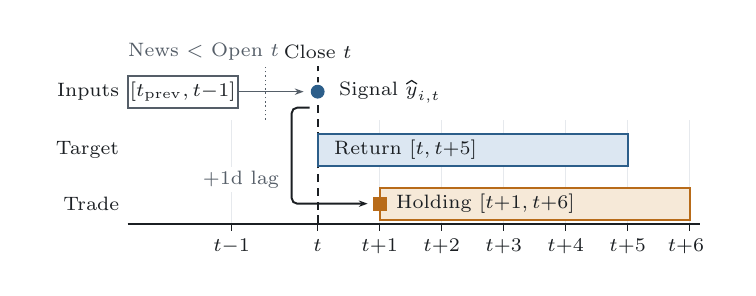
\begin{tikzpicture}[x=1in, y=1in]
  \useasboundingbox (0,0) rectangle (3.5030in, 1.20in);
  \fill[white] (0,0) rectangle (3.5030, 1.20);

  \foreach \gx in {1.02, 1.76, 2.07, 2.38, 2.69, 3.00, 3.31} {
    \draw[faint, line width=0.45pt] (\gx, 0.22) -- (\gx, 0.74);
  }
  \draw[slate, line width=0.55pt, densely dotted] (1.19, 0.74) -- (1.19, 1.01);
  \draw[ink, line width=0.75pt, densely dashed] (1.45, 0.22) -- (1.45, 1.01);

  \node[anchor=west, inner sep=0pt] at (0.50, 1.08) {\pfslate{News $<$ Open $t$}};
  \node[anchor=center, inner sep=0pt] at (1.45, 1.08) {\pfsub{Close $t$}};

  \node[anchor=east, inner sep=0pt] at (0.46, 0.88) {\pfsub{Inputs}};
  \node[anchor=east, inner sep=0pt] at (0.46, 0.59) {\pfsub{Target}};
  \node[anchor=east, inner sep=0pt] at (0.46, 0.32) {\pfsub{Trade}};

  % Inter-session news [t_prev, t-1] -> close-t forecast y_hat_{i,t} -> [t+1, t+6] holding
  \draw[slate, fill=white, line width=0.65pt] (0.50, 0.80) rectangle (1.05, 0.96);
  \node[anchor=center, inner sep=0pt] at (0.775, 0.88) {\pfsub{$[t_{\mathrm{prev}}, t{-}1]$}};

  \draw[pfmutedarrow] (1.05, 0.88) -- (1.38, 0.88);
  \fill[white] (1.45, 0.88) circle[radius=3.4pt];
  \fill[quantum] (1.45, 0.88) circle[radius=2.5pt];
  \node[anchor=west, fill=white, inner sep=1.8pt] at (1.53, 0.88) {\pfsub{Signal $\haty_{i,t}$}};

  \fill[white] (1.45, 0.51) rectangle (3.00, 0.67);
  \fill[quantumpale] (1.45, 0.51) rectangle (3.00, 0.67);
  \draw[quantum, line width=0.70pt] (1.45, 0.51) rectangle (3.00, 0.67);
  \node[anchor=west, inner sep=0pt] at (1.53, 0.59) {\pfsub{Return $[t, t{+}5]$}};

  \draw[ink, line width=0.70pt, rounded corners=2pt, -{Stealth[length=3.2pt, width=2.3pt]}]
    (1.41, 0.80) -- (1.32, 0.80) -- (1.32, 0.32) -- (1.70, 0.32);
  \node[anchor=east, fill=white, inner sep=1.5pt] at (1.28, 0.44) {\pfslate{$+1$d lag}};

  \fill[white] (1.76, 0.24) rectangle (3.31, 0.40);
  \fill[ochrepale] (1.76, 0.24) rectangle (3.31, 0.40);
  \draw[ochre, line width=0.75pt] (1.76, 0.24) rectangle (3.31, 0.40);
  \fill[ochre] (1.725, 0.285) rectangle (1.795, 0.355);
  \node[anchor=west, inner sep=0pt] at (1.84, 0.32) {\pfsub{Holding $[t{+}1, t{+}6]$}};

  \draw[ink, line width=0.60pt] (0.50, 0.22) -- (3.36, 0.22);
  \foreach \tx/\tlbl in {
    1.02/{$t{-}1$}, 1.45/{$t$}, 1.76/{$t{+}1$}, 2.07/{$t{+}2$},
    2.38/{$t{+}3$}, 2.69/{$t{+}4$}, 3.00/{$t{+}5$}, 3.31/{$t{+}6$}
  } {
    \draw[ink, line width=0.55pt] (\tx, 0.22) -- (\tx, 0.185);
    \node[anchor=north, inner sep=0pt] at (\tx, 0.145) {\pfsub{\tlbl}};
  }
\end{tikzpicture}
\end{document}
